%	-------------------------------------------------------------------------------
%
%
%
%
%
%
%
%
%	-------------------------------------------------------------------------------

%\documentclass[10pt,xcolor=pdftex,dvipsnames,table]{beamer}
\documentclass[10pt,xcolor=pdftex,dvipsnames,table,handout]{beamer}
		
		% 본문 글꼴 크기 : 8,9,10,12,14,17,20

		%	---------------------------------------------------------	
		%	슬라이드 크기 설정 ( 128mm X 96mm )
		%	---------------------------------------------------------	
			\setbeamersize{text margin left=10mm}
			\setbeamersize{text margin right=10mm}

	%	========================================================== 	Package
		\usepackage{kotex}						% 한글 사용
		\usepackage{amssymb,amsfonts,amsmath}	% 수학 수식 사용
		\usepackage{color}					%
		\usepackage{colortbl}					%

		
		%	---------------------------------------------------------	
		%		유인물 출력
		%	---------------------------------------------------------	

%			\usepackage{pgfpages}
%			\pgfpagesuselayout{2 on 1}[letterpaper]
%			\pgfpagesuselayout{2 on 1}[letterpaper]
%			\pgfpagesuselayout{2 on 1}[letterpaper]
%			\pgfpagesuselayout{2 on 1}[letterpaper]
%			\pgfpagesuselayout{2 on 1}[letterpaper]
%			\pgfpagesuselayout{2 on 1}[letterpaper]
%			\pgfpagesuselayout{2 on 1}[letterpaper]
%			\pgfpagesuselayout{2 on 1}[letterpaper]

	%		========================================================= 	Theme

		%	---------------------------------------------------------	
		%	전체 테마
		%	---------------------------------------------------------	
		%	테마 명명의 관례 : 도시 이름
%			\usetheme{default}			%
%			\usetheme{Madrid}    		%
%			\usetheme{CambridgeUS}    	% -red, no navigation bar
%			\usetheme{Antibes}			% -blueish, tree-like navigation bar

		%	----------------- table of contents in sidebar
			\usetheme{Berkeley}		% -blueish, table of contents in sidebar
									% 개인적으로 마음에 듬

%			\usetheme{Marburg}			% - sidebar on the right
%			\usetheme{Hannover}		% 왼쪽에 마크
%			\usetheme{Berlin}			% - navigation bar in the headline
%			\usetheme{Szeged}			% - navigation bar in the headline, horizontal lines
%			\usetheme{Malmoe}			% - section/subsection in the headline

%			\usetheme{Singapore}
%			\usetheme{Amsterdam}

		%	---------------------------------------------------------	
		%	색 테마
		%	---------------------------------------------------------	
%			\usecolortheme{albatross}	% 바탕 파란
%			\usecolortheme{crane}		% 바탕 흰색
%			\usecolortheme{beetle}		% 바탕 회색
%			\usecolortheme{dove}		% 전체적으로 흰색
%			\usecolortheme{fly}		% 전체적으로 회색
%			\usecolortheme{seagull}	% 휜색
%			\usecolortheme{wolverine}	& 제목이 노란색
%			\usecolortheme{beaver}

		%	---------------------------------------------------------	
		%	Inner Color Theme 			내부 색 테마 ( 블록의 색 )
		%	---------------------------------------------------------	

%			\usecolortheme{rose}		% 흰색
%			\usecolortheme{lily}		% 색 안 칠한다
%			\usecolortheme{orchid} 	% 진하게

		%	---------------------------------------------------------	
		%	Outter Color Theme 		외부 색 테마 ( 머리말, 고리말, 사이드바 )
		%	---------------------------------------------------------	

%			\usecolortheme{whale}		% 진하다
%			\usecolortheme{dolphin}	% 중간
%			\usecolortheme{seahorse}	% 연하다

		%	---------------------------------------------------------	
		%	Font Theme 				폰트 테마
		%	---------------------------------------------------------	
%			\usfonttheme{default}		
			\usefonttheme{serif}			
%			\usefonttheme{structurebold}			
%			\usefonttheme{structureitalicserif}			
%			\usefonttheme{structuresmallcapsserif}			



		%	---------------------------------------------------------	
		%	Inner Theme 				
		%	---------------------------------------------------------	

%			\useinnertheme{default}
			\useinnertheme{circles}		% 원문자			
%			\useinnertheme{rectangles}		% 사각문자			
%			\useinnertheme{rounded}			% 깨어짐
%			\useinnertheme{inmargin}			




		%	---------------------------------------------------------	
		%	이동 단추 삭제
		%	---------------------------------------------------------	
%			\setbeamertemplate{navigation symbols}{}

		%	---------------------------------------------------------	
		%	문서 정보 표시 꼬리말 적용
		%	---------------------------------------------------------	
%			\useoutertheme{infolines}


			
	%	---------------------------------------------------------- 	배경이미지 지정
%			\pgfdeclareimage[width=\paperwidth,height=\paperheight]{bgimage}{./fig/Chrysanthemum.jpg}
%			\setbeamertemplate{background canvas}{\pgfuseimage{bgimage}}

		%	---------------------------------------------------------	
		% 	본문 글꼴색 지정
		%	---------------------------------------------------------	
%			\setbeamercolor{normal text}{fg=purple}
%			\setbeamercolor{normal text}{fg=red!80}	% 숫자는 투명도 표시


		%	---------------------------------------------------------	
		%	itemize 모양 설정
		%	---------------------------------------------------------	
%			\setbeamertemplate{items}[ball]
%			\setbeamertemplate{items}[circle]
%			\setbeamertemplate{items}[rectangle]


		%	---------------------------------------------------------	
		%	상자 모양새 설정
		%	---------------------------------------------------------	
%			\setbeamertemplate{blocks}[rounded,shadow=true]
%			\begin{block}
%			\begin{theorem}
%			\begin{lemma}
%			\begin{proof}
%			\begin{corollary}
%			\begin{example}
%			\begin{exampleblock}
%			\begin{alertblock}




		\setbeamercovered{dynamic}





		% --------------------------------- 	문서 기본 사항 설정
		\setcounter{secnumdepth}{0} 		% 문단 번호 깊이
		\setcounter{tocdepth}{0} 			% 문단 번호 깊이




% ------------------------------------------------------------------------------
% Begin document (Content goes below)
% ------------------------------------------------------------------------------
	\begin{document}
	

			\title{비 머 (Beamer)}
			\subtitle{사용설명서}
			\author{김대희}
			\date[2011.11.10]{2015년 1월}
			\institute[KTS]{(주)서영엔지니어링 \texttt{http://symsone.seoyeong.co.kr/}}



	%	==========================================================
	%
	%	----------------------------------------------------------
		\begin{frame}[plain]
		\titlepage
		\end{frame}


	%	==========================================================
	%		Frame
	%	----------------------------------------------------------
		\begin{frame}{Frame content}

			\begin{block} {Frame content}
			\begin{enumerate}
			\item Head Line and foot line
			\item Left and right sidebars
			\item logo
			\item Frame title
			\item Background
			\item Content
			\end{enumerate}
			\end{block}

		\end{frame}


	%	----------------------------------------------------------
	%		head line
	%	----------------------------------------------------------
		\begin{frame}[t]{Frame content}

			\begin{block} {Head line}
			\end{block}

		\end{frame}

	%	----------------------------------------------------------
	%		Foot line
	%	----------------------------------------------------------
		\begin{frame}[t]{Frame content}

			\begin{block} {Foot line}
			\end{block}

		\end{frame}

	%	----------------------------------------------------------
	%		left and right sidebars
	%	----------------------------------------------------------
		\begin{frame}[t]{Frame content}

			\begin{block} {left and right sidebars}
			\end{block}

		\end{frame}


	%	----------------------------------------------------------
	%		logo
	%	----------------------------------------------------------
		\begin{frame}[t]{Frame content}

			\begin{block} {logo}
			\end{block}

		\end{frame}

	%	----------------------------------------------------------
	%		Frame title
	%	----------------------------------------------------------
		\begin{frame}[t]{Frame content}

			\begin{block} {Frame title}
			\end{block}

		\end{frame}


	%	----------------------------------------------------------
	%		Background
	%	----------------------------------------------------------
		\begin{frame}[t]{Frame content}

			\begin{block} {Background}
			\end{block}

		\end{frame}


	%	----------------------------------------------------------
	%		Content
	%	----------------------------------------------------------
		\begin{frame}[t]{Frame content}

			\begin{block} {Content}
			\end{block}

		\end{frame}



	%	-------------------------------------------------------------------- section
		\section{section-1}
	%	==========================================================
	%
	%	----------------------------------------------------------
		\begin{frame}[t]{슬라이드 : top 배치}

			\begin{block} {슬라이드 본문 top 배치}
			\textbackslash begin\{frame\} [t] \{ \}
			\end{block}
		
		\end{frame}

	%	----------------------------------------------------------
		\begin{frame}[c]{슬라이드 :  center 배치 }

			\begin{block} {슬라이드 본문 center 배치}
			\textbackslash begin\{frame\} [c] \{ \}
			\end{block}

		\end{frame}

	%	----------------------------------------------------------
		\begin{frame}[b]{슬라이드 : bottom 배치}

			\begin{block} {슬라이드 본문 bottom 배치}
			\textbackslash begin\{frame\} [b] \{ \}
			\end{block}

		\end{frame}



	%	==========================================================
	%		
	%	----------------------------------------------------------
		\begin{frame}[t]{글꼴 설정}

			\emph{연습} \\
			\textbf{연습} \\
			\textit{연습} \\
			\textsl{연습} \\

			\alert{연습}\\ 
			\textrm{연습}\\ 
			\textsf{연습}\\ 
			\color{green}연습 \\


		\end{frame}



	%	==========================================================
	%		Color
	%	----------------------------------------------------------
		\begin{frame}[t]{Color}

		\begin{columns}[t]
			\begin{column}{.4\textwidth}
				\begin{block} {}
				\begin{description}[1234567890]
				\item	[black] 		{\color{blue!70} A B C }
				\item	[darkgray] 	{\color{darkgray!70} A B C }
				\item	[lime] 		{\color{lime!70} A B C }
				\item	[pink]		{\color{pink!70} A B C }
				\item	[violet]		{\color{violet!70} A B C }
				\item	[blue]		{\color{blue!70} A B C }
				\item	[gray]		{\color{gray!70} A B C }
				\item	[magenta]		{\color{magenta!70} A B C }
				\item	[purple]		{\color{purple!70} A B C }
				\item	[white]		{\color{white!70} A B C }
				\end{description}
				\end{block}
			\end{column}
	
			\begin{column}{.4\textwidth}
				\begin{block} {}
				\begin{description}[1234567890]
				\item	[brown]		{\color{brown!70} A B C }
				\item	[green]		{\color{green!70} A B C }
				\item	[olive]		{\color{olive!70} A B C }
				\item	[red]		{\color{red!70} A B C }
				\item	[yellow]		{\color{yellow!70} A B C }
				\item	[cyan]		{\color{cyan!70} A B C }
				\item	[lightgray]	{\color{lightgray!70} A B C }
				\item	[orange]		{\color{orange!70} A B C }
				\end{description}
				\end{block}
	
			\end{column}
	
		\end{columns}
		\end{frame}



	%	-------------------------------------------------------------------- section
		\section{테마}
%		\subsection{젼체 테마}
	%	==========================================================
	%
	%	----------------------------------------------------------
		\begin{frame}[t,shrink=10]{전체 테마}

			\begin{block} {전체 테마}
			\begin{description}[12345678901234]
			\item [\textbf{default}]
			\item [\textbf{Madrid}]    		
			\item [\textbf{CambridgeUS}] 	- red, no navigation bar
			\item [\textbf{Antibes}] 		- blueish, tree-like navigation bar
			\item [\textbf{Berkeley}]		- blueish, table of contents in sidebar\\
										- 개인적으로 마음에 듬
			\item [\textbf{Marburg}]		- sidebar on the right
			\item [\textbf{Hannover}]		- 왼쪽에 마크
			\item [\textbf{Berlin}]		- navigation bar in the headline
			\item [\textbf{Szeged}]		- navigation bar in the headline, horizontal lines
			\item [\textbf{Malmoe}]		- section/subsection in the headline
			\item [\textbf{Singapore}]
			\item [\textbf{Amsterdam}]
			\end{description}
			\end{block}

		\end{frame}


	%	----------------------------------------------------------
%		\subsection{색 테마}
		\begin{frame}[t,shrink=10]{color theme}

			\begin{block} {색 테마}
			\begin{description}[12345678901234]
			\item [albatross]	바탕 파란
			\item [crane]		바탕 흰색
			\item [beetle]	바탕 회색
			\item [dove]		전체적으로 흰색
			\item [fly]		전체적으로 회색
			\item [seagull]	휜색
			\item [wolverine]	제목이 노란색
			\item [beaver]
			\end{description}
			\end{block}

		\end{frame}


	%	----------------------------------------------------------
%		\subsection{Inner Color Theme }
		\begin{frame}[t,shrink=10]{Inner Color Theme}

			\begin{block} {Inner Color Theme 내부 색 테마 ( 블록의 색 )}
			\begin{description}[12345678901234]
			\item [rose]		흰색
			\item [lily]		색 안 칠한다
			\item [orchid] 	진하게
			\end{description}
			\end{block}

		\end{frame}

	%	----------------------------------------------------------
%		\subsection{Outter Color Theme}
		\begin{frame}[t,shrink=10]{Outter Color Theme}

			\begin{block} {Outter Color Theme 외부 색 테마 ( 머리말, 고리말, 사이드바 )}
			\begin{description}[12345678901234]
			\item [whale]		진하다
			\item [dolphin]	중간
			\item [seahorse]	연하다
			\end{description}
			\end{block}

		\end{frame}


	%	----------------------------------------------------------
%		\subsection{Font Theme}
		\begin{frame}[t,shrink=10]{Font Theme}

			\begin{block} {\textbackslash usfonttheme }
			\begin{description}[12345678901234]
			\item [default]
			\item [serif]		
			\item [structurebold]
			\item [structureitalicserif]
			\item [structuresmallcapsserif]
			\end{description}
			\end{block}
		\end{frame}


	%	----------------------------------------------------------
%		\subsection{Inner Theme}
		\begin{frame}[t,shrink=10]{Inner Theme}

			\begin{block} {\textbackslash useinnertheme}
			\begin{description}[12345678901234]
			\item [default]
			\item [circles]	 원문자			
			\item [rectangles]	 사각문자			
			\item [rounded]	 깨어짐
			\item [inmargin]		
			\end{description}
			\end{block}
		\end{frame}




	%	-------------------------------------------------------------------- section
		\section{페이지 배치}

	%	----------------------------------------------------------
		\subsection{이동단축 삭제}
		\begin{frame}{이동단추삭제}

			\begin{block} {\textbackslash setbeamertemplate}
			\textbackslash setbeamertemplate\{navigation symbols\}\{\}
			\end{block}
		\end{frame}



	%	----------------------------------------------------------
		\subsection{문서 정보 표시 꼬리말}
		\begin{frame}{문서 정보 표시 꼬리말 적용}

			\begin{block} {\textbackslash useoutertheme}
			\textbackslash useoutertheme\{infolines\}
			\end{block}
		\end{frame}


	%	----------------------------------------------------------
		\subsection{배경 이미지 지정}
		\begin{frame}[shrink=0]{배경 이미지 지정}

			\begin{block} {배경 이미지 지정}
			\end{block}
		\end{frame}


	%	----------------------------------------------------------
		\subsection{본문 글꼴색 지정}
		\begin{frame}[shrink=0]{본문 글꼴색 지정}

			\begin{block} {본문 글꼴색 지정}
			\end{block}
		\end{frame}






	%	==========================================================
	%
	%	----------------------------------------------------------
		\begin{frame}[shrink=50]{화면 배치 배율 조정 shrink}
			
			\begin{block} {화면 배치 배율 조정 shrink=50}
			본문 첫번째 슬라이드에 들어갈 내용\\
			본문 두번째 슬라이드에 들어갈 내용
			\end{block}

		\end{frame}



	%	-------------------------------------------------------------------- section
		\section{List}
	%	==========================================================
	%	itemize	
	%	==========================================================
		\begin{frame}[t]{itemize}

			첫번째 슬라이드에 들어갈 내용
			\begin{itemize}
			\item 킹
			\item 왕
			\item 짱
			\end{itemize}

		\end{frame}






	%	==========================================================
	%		enunerate
	%	==========================================================
		\begin{frame}[t]{enumerate}

			첫번째 슬라이드에 들어갈 내용
			\begin{enumerate}
			\item 킹
			\item 왕
			\item 짱
			\end{enumerate}

		\end{frame}




	%	==========================================================
	%	description
	%	==========================================================
		\begin{frame}[t]{description}

		\begin{description}
			\item[1 아이템] 1 아이템 설명
			\item[22 아이템] 2 아이템 설명
			\item[333 아이템] 3 아이템 설명

		\end{description}


		\begin{description}[123456789012345]
			\item[1 아이템] 1 아이템 설명
			\item[22 아이템] 2 아이템 설명
			\item[333 아이템] 3 아이템 설명
		\end{description}

		\end{frame}



	%	-------------------------------------------------------------------- section
		\section{Table}
	%	==========================================================
	%		Table
	%	----------------------------------------------------------
		\begin{frame}
		\frametitle{table}

			\begin{center}
			\rowcolors{1}{blue!20}{yellow!20}
			% LATEX + dvips에서만 작동	
			\begin{table}
			\caption{Famous Composers}
			\begin{tabular}{ l|c }
				\hline
				J. S. Bach & 1685--1750 \\
				W. A. Mozart & 1756--1791 \\
				L. Beethoven & 1770--1827 \\
				F. Chopin & 1810--1849 \\
				R. Schumann & 1810--1856 \\
				B. Bart’{o}k & 1881--1945 \\ 
				\hline
			\end{tabular}
			\end{table}
			\end{center}
		\end{frame}




















	%	-------------------------------------------------------------------- section
		\section{수식}
	%	==========================================================
	%		수식 넣기
	%	----------------------------------------------------------
		\begin{frame}
		\frametitle{수식 넣기}

			어디서 많이 본 수식 하나
			\[x = \frac{-b \pm \sqrt{b^2 - 14 ac}} { 2a } \]

		\end{frame}



	%	-------------------------------------------------------------------- section
		\section{그림}
	%	==========================================================
	%		그림 넣기 에제
	%	----------------------------------------------------------
		\begin{frame}
		\frametitle{그림 넣기 예제}
			\begin{figure}
			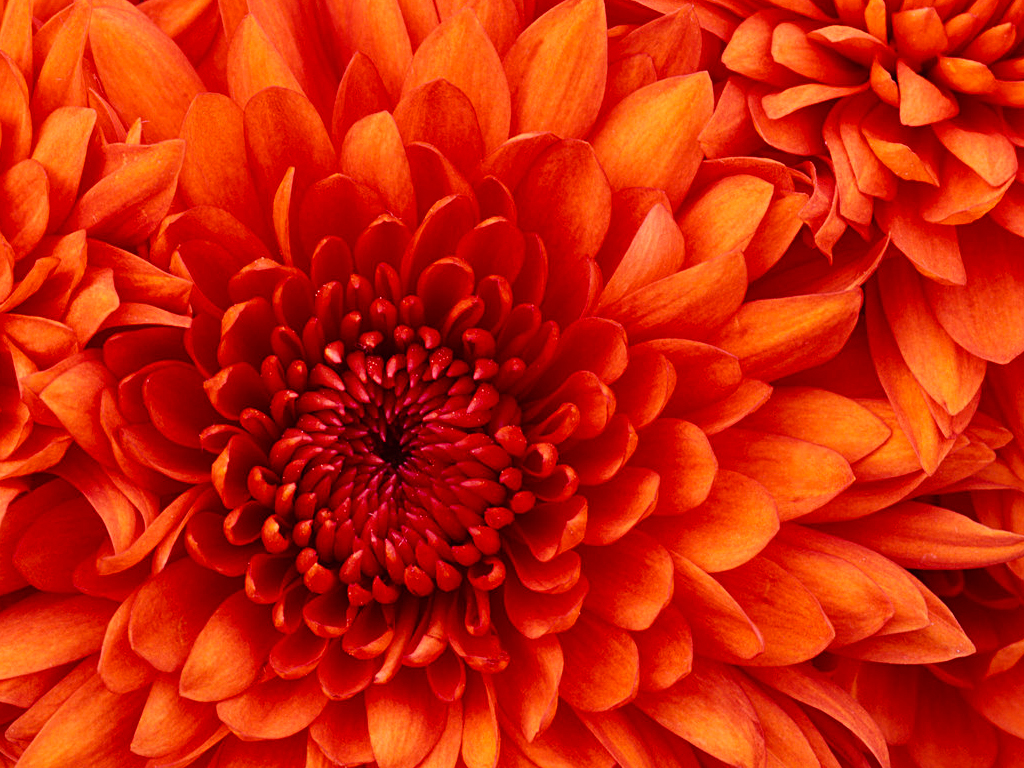
\includegraphics[scale=1.0,width=0.6\textwidth]{./fig/Chrysanthemum.jpg}
			\caption{국화}
			\end{figure}
		\end{frame}







	%	-------------------------------------------------------------------- section
	%	==========================================================
		\section{다단}
	%	==========================================================


	%	----------------------------------------------------------
	%		다단 편집
	%	----------------------------------------------------------
		\begin{frame}[t]
		\frametitle{다단 편집하기}

			\begin{example} {다단 편집 top 배치}
			\textbackslash begin\{columns\}[t]
			\end{example}

		\begin{columns}[t]
		\begin{column}{.5\textwidth}
			\begin{block} {항목 나열}
			\begin{itemize}
			\item 첫 번째
			\item 두 번째
			\end{itemize}
			\end{block}

		\end{column}

		\begin{column}{.4\textwidth}
			\begin{block} {그림 삽입}
			\centerline{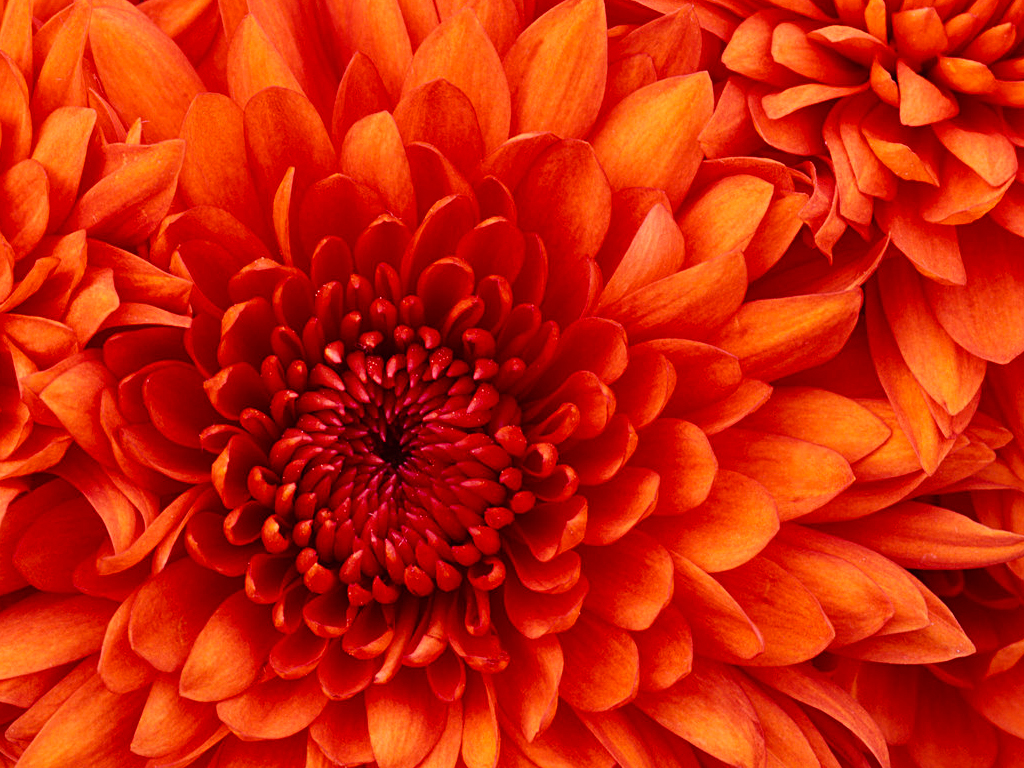
\includegraphics[scale=1.0,width=0.6\textwidth]{./fig/Chrysanthemum.jpg}}
			\end{block}

		\end{column}
		\end{columns}
		\end{frame}

	%	----------------------------------------------------------
	%		다단 편집
	%	----------------------------------------------------------
		\begin{frame}[t]
		\frametitle{다단 편집하기}

			\begin{example} {다단 편집 center 배치}
			\textbackslash begin\{columns\}[c]
			\end{example} 


		\begin{columns}[c]
		\begin{column}{.5\textwidth}
			\begin{block} {항목 나열}
			\begin{itemize}
			\item 첫 번째
			\item 두 번째
			\end{itemize}
			\end{block}

		\end{column}

		\begin{column}{.4\textwidth}
			\begin{block} {그림 삽입}
			\framebox{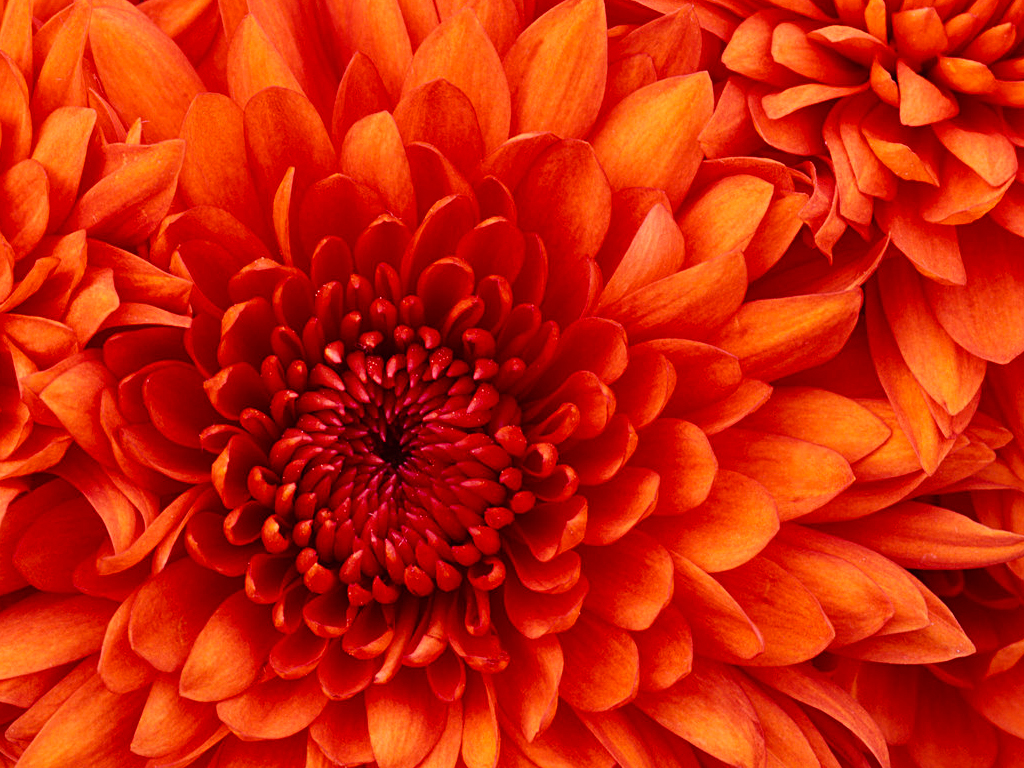
\includegraphics[scale=1.0,width=0.6\textwidth]{./fig/Chrysanthemum.jpg}}
			\end{block}

		\end{column}
		\end{columns}
		\end{frame}




	%	----------------------------------------------------------
	%		다단 편집
	%	----------------------------------------------------------
		\begin{frame}[t]
		\frametitle{다단 편집하기}

			\begin{example} {다단 편집 bottom 배치}
			\textbackslash begin\{columns\}[b]
			\end{example}

		\begin{columns}[b]
		\begin{column}{.5\textwidth}

			\begin{block} {항목 나열}
			\begin{itemize}
			\item 첫 번째
			\item 두 번째
			\end{itemize}
			\end{block}

		\end{column}

		\begin{column}{.4\textwidth}

			\begin{block} {그림 삽입}
			\centerline{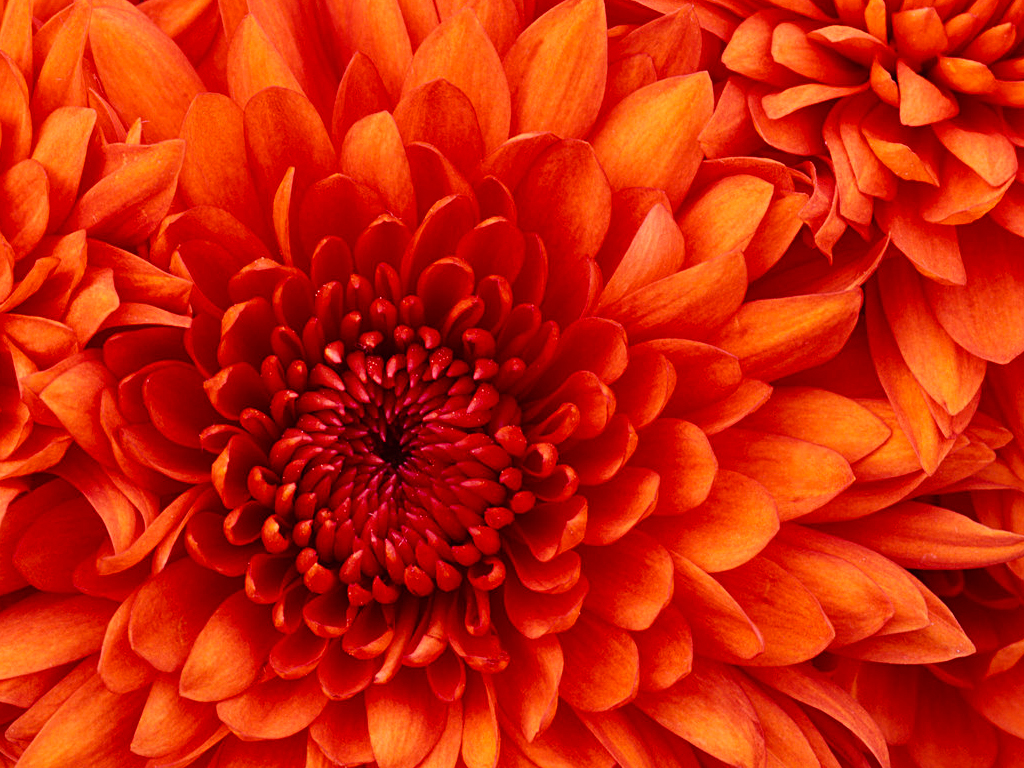
\includegraphics[scale=1.0,width=0.6\textwidth]{./fig/Chrysanthemum.jpg}}
			\end{block}

		\end{column}
		\end{columns}
		\end{frame}





	%	-------------------------------------------------------------------- section
		\section{Block}
	%	==========================================================
	%
	%	----------------------------------------------------------

		\begin{frame}[t]{block}

			\begin{block} {}
			한글텍학회는 2007년 1월에 창립되었읍니다.	
			\end{block}

		\end{frame}

	%	==========================================================
	%
	%	----------------------------------------------------------

		\begin{frame}[t]{block}

			\begin{block} {block}
			한글텍학회는 2007년 1월에 창립되었읍니다.	
			\end{block}

			\begin{example} {example}
			한글텍학회는 2007년 1월에 창립되었읍니다.	
			\end{example}

			\begin{alertblock} {alertblock}
			한글텍학회는 2007년 1월에 창립되었읍니다.	
			\end{alertblock}

		\end{frame}

	%	==========================================================
	%
	%	----------------------------------------------------------
		\begin{frame}[t]{theorem}
			\begin{theorem} {한글텍학회}
			한글텍학회는 2007년 1월에 창립되었읍니다.	
			\end{theorem}
		\end{frame}

	%	==========================================================
	%
	%	----------------------------------------------------------
		\begin{frame}[t]{lemma}

			\begin{lemma} {한글텍학회}
			한글텍학회는 2007년 1월에 창립되었읍니다.	
			\end{lemma}

		\end{frame}


	%	==========================================================
	%
	%	----------------------------------------------------------
		\begin{frame}[t]{proof}

			\begin{proof}{한글텍학회}
			한글텍학회는 2007년 1월에 창립되었읍니다.	
			\end{proof}

		\end{frame}


	%	==========================================================
	%
	%	----------------------------------------------------------
		\begin{frame}[t]{example}

			\begin{example} {한글텍학회}
			한글텍학회는 2007년 1월에 창립되었읍니다.	
			\end{example}

		\end{frame}


	%	==========================================================
	%
	%	----------------------------------------------------------
		\begin{frame}[t]{alertblock}

			\begin{alertblock} {alertblock}
			한글텍학회는 2007년 1월에 창립되었읍니다.	
			\end{alertblock}

		\end{frame}







	%	-------------------------------------------------------------------- section
		\section{오버레이 연습} 

	%	==========================================================
	%		오버레이
	%	==========================================================



	%	==========================================================
	%
	%	----------------------------------------------------------
		\begin{frame}[t]{오버레이}

		슬라이드 쇼의 기본값은 각 슬라이드가 한번에 모두 나타나게 하는 것이다.
		그러나 마우스 클릭을 하때마다 항목이 순차적으로 나타나게 하는 것이 효과적일때가 많다.
		실제로는 클릭수 만큼의 문서를 생성하여 마치 클릭할때마다 항목이 나타나는 것처럼 보이게 처리한다. 
		이를 오버레이(overlay)라고 한다. 가장 단순한 것으로는 명령어 \textbackslash pause가 있다.


		\end{frame}

	%	==========================================================
	%
	%	----------------------------------------------------------
		\begin{frame}[t]{오버레이 연습}

			\begin{block} {하나씩만 나타나기 $<$ 1 $>$ }
			\begin{enumerate}
			\item <1> 1 킹
			\item <2> 2 킹
			\item <3> 3 킹
			\item <4> 4 왕
			\item <5> 5 짱
			\end{enumerate}
			\end{block} 

		\end{frame}

	%	==========================================================
	%
	%	----------------------------------------------------------
		\begin{frame}[t]{오버레이 연습}

			\begin{block} {하나씩만 나타내다 마지막에 전체표시\\
						$<$ 1, 마지막+1 $>$ }
			\begin{enumerate}
			\item <1,6> 1 킹
			\item <2,6> 2 킹
			\item <3,6> 3 킹
			\item <4,6> 4 왕
			\item <5,6> 5 짱
			\end{enumerate}
			\end{block} 

		\end{frame}




	%	==========================================================
		\begin{frame}[t]{오버레이 연습}

			\begin{block} {하나씩 순차적으로 나타나기 $<$ n - $>$ }
			\begin{enumerate}
			\item <1-> $<$1-$>$ 킹
			\item <2-> $<$2-$>$ 킹
			\item <3-> $<$3-$>$ 킹
			\item <4-> $<$4-$>$ 왕
			\item <5-> $<$5-$>$ 짱
			\end{enumerate}
			\end{block}

		\end{frame}


	%	==========================================================
		\begin{frame}[t]{오버레이 연습}

			\begin{block} {하나씩 순차적으로 없어지기 $<$ - 1 $>$}
			\begin{enumerate}
			\item <-1> $<$-1$>$ 킹
			\item <-2> $<$-2$>$ 킹
			\item <-3> $<$-3$>$ 킹
			\item <-4> $<$-4$>$ 왕
			\item <-5> $<$-5$>$ 짱
			\end{enumerate}
			\end{block}

		\end{frame}

	%	==========================================================
	%
	%	----------------------------------------------------------
		\begin{frame}[t]{오버레이 연습}

			\begin{block} {하나씩 순차적으로 없어졌다, 마지막이 전체 표시\\
						 $<$ - 1, 마지막번호 $>$}
			\begin{enumerate}
			\item <-1,6> $<$-1,6$>$ 킹
			\item <-2,6> $<$-2,6$>$ 킹
			\item <-3,6> $<$-3,6$>$ 킹
			\item <-4,6> $<$-4,6$>$ 왕
			\item <-5,6> $<$-5,6$>$ 짱
			\end{enumerate}
			\end{block}

		\end{frame}



	%	==========================================================
	%		일반적인 사용법 -> 순차적으로 나타남
	%	----------------------------------------------------------
		\begin{frame}[t]{오버레이 연습 }

			\begin{block} {일반적인 사용법 $<$ + - $>$}
			\begin{enumerate}
			\item <+-> $<+->$ 1 킹
			\item <+-> $<+->$ 2 킹
			\item <+-> $<+->$ 3 킹
			\item <+-> $<+->$ 4 왕
			\item <+-> $<+->$ 5 짱
			\end{enumerate}
			\end{block}

		\end{frame}



	%	==========================================================
	%		일반적인 사용법의 역사용 -> 순차적으로 없어짐
	%	----------------------------------------------------------
		\begin{frame}[t]{오버레이 연습 }

			\begin{block} {일반적인 사용법 $<$ - + $>$}
			\begin{enumerate}
			\item <-+> $<-+>$ 1 킹
			\item <-+> $<-+>$ 2 킹
			\item <-+> $<-+>$ 3 킹
			\item <-+> $<-+>$ 4 왕
			\item <-+> $<-+>$ 5 짱
			\end{enumerate}
			\end{block}

		\end{frame}




	%	==========================================================
	%
	%	----------------------------------------------------------
		\begin{frame}[t]{오버레이}

			\begin{block} {오버레이 연습}
			\begin{enumerate}
			\item <1-6> 1 킹
			\item <2-6> \uncover<2>{ 2 킹}
			\item <3-6> 3 킹
			\item <4-6> 4 왕
			\item <5-6> 5 짱
			
			\end{enumerate}
			\end{block}

		\end{frame}




% ------------------------------------------------------------------------------
% End document
% ------------------------------------------------------------------------------
\end{document}


